\PassOptionsToPackage{utf8x}{inputenc}
% JuliaCon proceedings template
\documentclass{juliacon}
\usepackage{hyperref}
\usepackage{jlcode}

\usepackage[mathletters]{ucs} 
\usepackage[utf8x]{inputenc}
% suggested by https://discourse.julialang.org/t/what-do-you-use-to-embed-julia-code-in-latex/23992/2


\usepackage[dvipsnames,table]{xcolor}  % Coloured text etc.
\usepackage{natbib}
\usepackage{amsmath}
\usepackage{nicefrac}
\setcitestyle{square,numbers}
\usepackage{hyperref}
\usepackage{cleveref}
\newcommand\myshade{85}
\colorlet{mylinkcolor}{violet}
\colorlet{mycitecolor}{YellowOrange}
\colorlet{myurlcolor}{Aquamarine}
\hypersetup{
    colorlinks=true,
    linkcolor  = mylinkcolor!\myshade!black,
    citecolor  = mycitecolor!\myshade!black,
    urlcolor   = myurlcolor!\myshade!black,
}

\newcommand{\params}{\mathbf{p}}
\newcommand{\stateVar}{\boldsymbol{u}}
\newcommand{\stateDisc}{\mathbf{u}}
\newcommand{\testFun}{\varphi}
\newcommand{\testFunMat}{\boldsymbol{\Phi}}
\newcommand{\stateMat}{\mathbf{U}}
\newcommand{\quadMat}{\mathbf{Q}}
\newcommand{\timeVec}{\mathbf{t}}


\DeclareMathOperator{\logdet}{logdet}
\DeclareMathOperator{\argmin}{argmin}
\DeclareMathOperator{\vecOp}{vec}

\lstset{
  columns=flexible,
  keepspaces=true
}

\setcounter{page}{1}

\begin{document}

% **************GENERATED FILE, DO NOT EDIT**************

\title{WENDy.jl}

\author[1]{Nicholas Rummel}
\author[1]{Stephen Becker}
\author[2]{Daniel Messenger}
\author[1]{Vanja Dukic}
\author[1]{David M. Bortz}
\affil[1]{University of Colorado Boulder}
\affil[2]{Los Alamos National Laboratory}

\keywords{Julia, Parameter Estimation, Optimization, Differential Equations}

\hypersetup{
pdftitle = {WENDy.jl},
pdfsubject = {JuliaCon 2025 Proceedings},
pdfauthor = {Nicholas Rummel, Stephen Becker, Daniel Messenger, Vanja Dukic, David M. Bortz},
pdfkeywords = {Julia, Parameter Estimation, Optimization, Differential Equations},
}



\maketitle

\section{Summary}

The Weak-form Estimation of Non-linear Dynamics (WENDy) framework is a recently developed approach for parameter estimation of systems of ordinary differential equations (ODEs). Prior work demonstrated WENDy to be robust, computationally efficient, and accurate, but only works for ODEs that are linear-in-parameters. All the algorithms in this package accommodate ODEs that are nonlinear-in-parameters. The WENDy-MLE algorithm in particular approximates a maximum likelihood estimator via local non-convex optimization methods; it has better accuracy, a substantially larger domain of convergence, and is often faster than other weak form methods and the conventional output error least squares method. 

The code was designed to provide a mostly automated process; this facilitates an application friendly interface. We utilize symbolic programming to obtain an analytic expressions for the likelihood function and its first and second order derivatives. Moreover, unlike the prior algorithms which focus only on additive Gaussian noise, we extend the framework to accommodate  data corrupted by either multiplicative log-normal noise or additive Gaussian noise. The \href{https://github.com/nrummel/WENDy.jl}{WENDy.jl} package efficiently and accessibly implements many weak form methods that were previously unavailable to the Julia community. 

\section{Statement of Need}
Julia has a bountiful ecosystem of numerical solvers that can directly solve ordinary differential equations \citep{BezansonEdelmanKarpinskiEtAl2017SIAMRev,RackauckasNie2017JORS}. Furthermore, considerable effort has been made to facilitate automatic differentiation \citep{RevelsLubinPapamarkou2016arXiv160707892}. This supports downstream optimization routines that can be used for control, optimal design, and, more pertinently to this work, parameter estimation. However, in spite of these efficiencies, using forward simulation at every iteration of an optimization routine can rapidly increase the computational cost, especially in high-dimensional or stiff systems. For chaotic systems, using forward simulation also can introduce numerical instability. In contrast, weak form methods do not suffer in this way. Thus, to tackle more challenging systems, alternative approaches such as weak form methods become attractive. These methods do not rely on forward simulation of the differential equations to accomplish estimation. Instead, by optimizing the \emph{equation error} rather than the \emph{output error}, weak form methods efficiently optimize the parameters irrespectively of the challenge of forward simulation of the system.

\section{Research Impact Statement}

Interest in weak form methods have been revitalized in the last decade \citep{MessengerTranDukicEtAl2024SIAMNews}. These methods are used in broader applications beyond parameter estimation; WSINDy uses sparse regularization to simultaneously identify the governing equations of ordinary differential equations \citep{MessengerBortz2021MultiscaleModelSimul} and partial differential equations \citep{MessengerBortz2021JComputPhys} that are linear in parameters. Furthermore, WSINDy has been used in conjunction with dimensionality reduction techniques to effectively identify reduced order models \citep{TranHeMessengerEtAl2024ComputMethodsApplMechEng}.
WENDy.jl brings many existing weak form methods \citep{BortzMessengerDukic2023BullMathBiol} into the Julia ecosystem as well as integrates novel approaches for systems that are non-linear in parameters and have an error structure beyond simple additive {\it iid}  Gaussian noise. 

Specifically, in this work we construct an analytic expression for an approximation of a likelihood function, build Julia functions for the likelihood, its first, and its second order derivatives with symbolic programming, and then perform second order optimization to estimate parameters. All algorithms were extended to accommodate systems of ordinary differential equations that are both linear or nonlinear in parameters. In the linear in parameters case, we leverage computational advantages where available. Also, the code effectively handles data that has been corrupted by both additive Gaussian and multiplicative LogNormal noise.

\section{Mathematics}

The underlying purpose of our approach is to obtain an estimator for unknown parameters $\params \in \mathbb{R}^J$ in an ordinary differential equation of the form 
\begin{equation} \label{eq:ode}
    \dot{\stateVar}(t) = \mathbf{f}(\stateVar, t, \params).
\end{equation}
Here, the right hand side function $\mathbf{f}: \mathbb{R}^D \times \mathbb{R} \times \mathbb{R}^J \rightarrow \mathbb{R}^D$  is defined on a compact domain $t\in [0,T]$ for state variable $\stateVar\in \mathbb{R}^D$, and  may be linear or nonlinear in $t,\stateVar,$ and $\params$.

The weak form of a differential equation is obtained by taking the inner product on both side of the equation with an arbitrary test function $\testFun$ along each dimension
\begin{equation}\label{eq:weakForm}
    - \langle\dot{\testFun}, \stateVar \rangle  = \langle \testFun, \mathbf{f}(\stateVar,\timeVec,\params) \rangle.
\end{equation}

Given data on a uniform grid $\bigl\{(\mathrm{t}_m, \mathrm{u}_m)\bigr\}_{m=0}^M$ and selecting specific test functions $\{\testFun\}_{k=1}^K$, the inner products can be approximated through quadrature. This can be written succinctly by introducing a data matrix $\stateMat \in \mathbb{R}^{(M+1)\times D}$, a test function matrix $\testFunMat \in \mathbb{R}^{K\times (M+1)}$, the matrix-valued function $\mathbf{F}: \mathbb{R}^{(M+1)\times D}\times \mathbb{R}^{M+1} \times \mathbb{R}^J \rightarrow \mathbb{R}^{(M+1)\times D}$ which naturally extends to $\mathbf{f}$, and a quadrature matrix $\quadMat\in \mathbb{R}^{(M+1)\times (M+1)}$
\begin{equation}\label{eq:weakFormDisc}
    - \testFunMat \quadMat \stateMat \approx \dot{\testFunMat} \quadMat \mathbf{F}(\stateMat,\timeVec,\params) .
\end{equation}
Moving all the parameters to the right hand side, we can define an expression for the \emph{weak residual} 
\begin{equation}\label{eq:wres}
    \mathbf{r}(\params) := \vecOp\left[\dot{\testFunMat} \quadMat \mathbf{F}(\stateMat,\timeVec,\params) + \testFunMat \quadMat \stateMat\right] \in \mathbb{R}^{KD}
\end{equation}
where $\vecOp$ vectorizes the matrix expression on the right hand side of \cref{eq:weakFormDisc}. Because the quadrature  \emph{approximates} the underlying integrals, and the data has been \emph{corrupted by noise}, one can expect $r$ to be \emph{small}, albeit not zero,  when evaluated at the true parameters.

By leveraging a known distribution of additive Gaussian noise and a linearization, one can obtain that the scaled weak residual is approximately distributed as a Gaussian 
\begin{equation}\label{eq:weakResDist}
   \mathbf{S}(\params)^{-\nicefrac{1}{2}} \mathbf{r}(\params) \stackrel{approx}{\sim} \mathcal{N}(0, I).
\end{equation}
where the specific form of the covariance matrix $\mathbf{S}$ and more details can be found in \citep{RummelMessengerBeckerEtAl2025arXiv250208881b}. A similar expression is obtained in the case of multiplicative Log-Normal noise. The WENDy-MLE algorithm leverages \cref{eq:weakResDist} to obtain the approximate maximum likelihood estimator (A-MLE) via optimization
\begin{equation}\label{eq:mle}
    \hat{\params} = \underset{\params}{\argmin}\Bigl( \logdet\bigl(\mathbf{S}(\params)\bigr) + \mathbf{r}(\params)^\top \mathbf{S}(\params)^{-1}\mathbf{r}(\params)\Bigr).
\end{equation}
Julia makes it possible to obtain first and second order derivatives of the objective function prior to performing optimization through symbolic computations and our custom implementation. This allows for efficient use of second order routines such as Trust Region methods. 

\section{Software Design}

\href{https://github.com/nrummel/WENDy.jl}{WENDy.jl} \citep{RummelMessengerBeckerEtAl2025arXiv250208881b} is the first implementation of these weak form methods in Julia. The package utilizes  other Julia packages such as \href{https://github.com/mcabbott/Tullio.jl}{Tullio.jl} \citep{Michael2026},  \href{https://github.com/JuliaSymbolics/Symbolics.jl}{Symbolics.jl} \citep{GowdaMaCheliEtAl2021ACMCommunComputAlgebra}, \href{https://github.com/SciML/Optim.jl}{Optim.jl} \citep{KMogensenNRiseth2018JOSS}, \href{https://github.com/JuliaSmoothOptimizers/JSOSolvers.jl}{JSOSolvers.jl} \citep{MigotOrbanSoaresSiqueira2024}, and \href{https://github.com/SciML/NonlinearSolve.jl}{NonlinearSolve.jl} \citep{PalHoltorfLarssonEtAl2024arXiv240316341} to aid in custom implementation of novel mathematical algorithms. The code was designed so that users can simply define a struct
% \vspace{.5cm}
\begin{jllisting}
    prob = WENDyProblem(
        tt::AbstractVector{<:Real}, 
        U::AbstractVecOrMat{<:Real}, 
        f::Function, 
        J::Int
    )
\end{jllisting}

The only required inputs are \texttt{tt}, \texttt{U}, \texttt{f}, and \texttt{J} which correspond to the vector of time points for the observation data, a matrix whose columns contain the observation data, the function that defines the differential equation of interest, and the number of parameters the user wishes to estimate, respectively. There are optional parameters that allow the user to specify more information, see our \href{https://nrummel.github.io/WENDy.jl/stable/}{documentation} for details.
%; in particular, if the function \texttt{f} is linear or nonlinear in the parameters, if the observation data \texttt{U} has been corrupted by additive Gaussian noise or multiplicative LogNormal noise, if the user wishes to override default parameters, or if constraints should be imposed on the parameter estimation problem. 

The WENDy.jl algorithms then build the necessary parameter estimation problem by first creating the necessary test function matrix, computing symbolic derivatives, and then building the Julia functions necessary to perform optimization. This all happens when the 
\texttt{WENDyProblem} % <-- Stephen's manual solution
%\hspace{-1cm}\jlinl{WENDyProblem}\hspace{-1cm} 
is constructed. Then, the user can solve the parameter estimation problem by calling 
\begin{jllisting}
    pHat = solve(
        wendyProb::WENDyProblem, 
        p0::AbstractVector{<:Real}
    )
\end{jllisting}
The user is expected to provide an initial guess \texttt{p0} for the parameters of interest.
%and optional overrides to default a parameter struct and an optimization algorithm. 

We focused on providing users with a simple software interface so the weak form algorithms can be used with as little expert knowledge as possible, with the hope that this will result in a broader appeal for weak form methods use in applications.

\section{Short Demonstration}

Consider the Logistic Growth equation 
\begin{equation} \label{eq:logisticGrowth}
     % \begin{aligned}
        \dot{u} = p_1 u - p_2 u^2 , t \in [0,T].\\
    % \end{aligned}
\end{equation}
Data is observed on a uniform grid $\bigl\{(m\Delta t, \mathrm{u}_m) \bigr\}_{m=0}^M$, the observations are corrupted by multiplicative noise 
\begin{equation*}
    \mathrm{u}_m = u(t_m) \eta_m, \; \forall m \in \{0,1,\cdots, M\}
\end{equation*}
where $\log(\eta_m) \stackrel{iid}{\sim} N(0, \rho^2)$, and the true parameters are $\params^* = [2.25, 7.0]^\top$. For the experiment shown below, the hyperparameters are set to $T = 10, M = 100, \Delta t = \nicefrac{1}{10}, \rho = \nicefrac{1}{2}$. One instance of the data, the estimated trajectory, and the true trajectory is plotted in \cref{fig:LogisticGrowth_TrajectoryWithData}.

\begin{figure}[ht!]
    \centering
    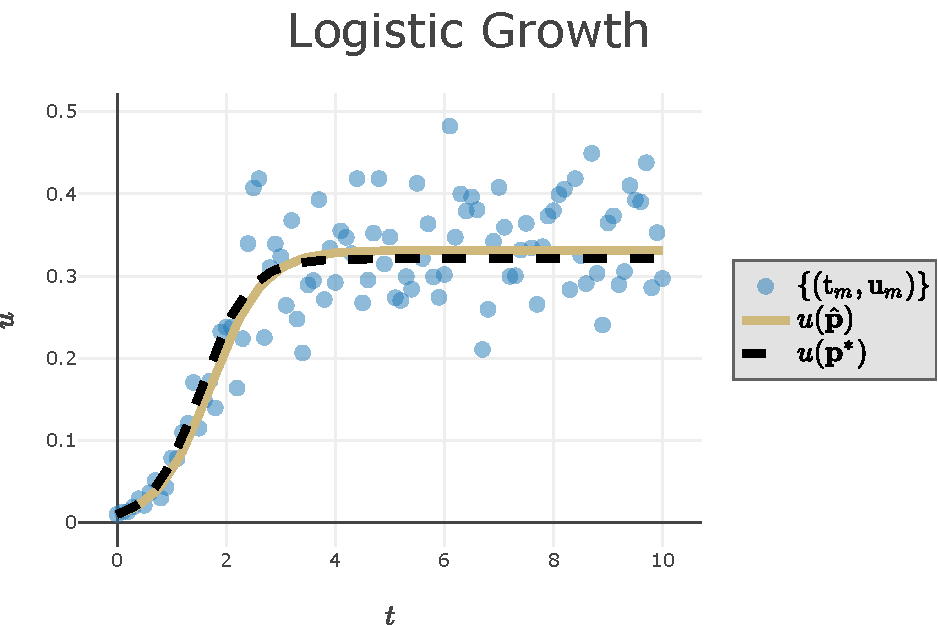
\includegraphics[width=\linewidth]{LogisticGrowth_TrajectoryWithData.pdf}
    \caption{WENDy.jl estimates the parameters given data corrupted with multiplicative noise. The observation data is shown with blue markers, the state's trajectory with the estimated parameters is shown with gold line, and the state's trajectory with the true parameters is shown with the dashed black line.}
    \label{fig:LogisticGrowth_TrajectoryWithData}
\end{figure}
WENDy.jl obtains the A-MLE from an initial guess of $\params_0 = [2.72, 3.67]^\top$ and performing optimization of \cref{eq:mle}. In this example, our estimated parameters have a coefficient relative error of 12\% and a relative average forward solve error of 4.1\%. As a quick point of reference, a standard output error least squares algorithm resulted in a coefficient relative error  14\% and a relative average forward solve error of 5.6\%. For more extensive examples, comparisons, and numerical results see \citep{RummelMessengerBeckerEtAl2025arXiv250208881b}.
% Figures can be included like this:
% ![Caption for example figure.\label{fig:example}](figure.png)
% and referenced from text using \autoref{fig:example}.

% Figure sizes can be customized by adding an optional second parameter:
% ![Caption for example figure.](figure.png){ width=20% }

\section{AI usage disclosure}

No generative AI tools were used in the development of this software, the writing
of this manuscript, or the preparation of supporting materials.

\section{Acknowledgements}

We acknowledge contributions from Jackson Krebsbach (University of Colorado), Will Houser (University of Colorado), April Tran (University of Colorado), and Lloyd Fung
(Imperial College) for insights regarding software development for weak form methods and mathematical rigor.

This work is supported in part by the National Institute of General Medical Sciences grant R35GM149335, National Science Foundation grant 
2109774, National Institute of Food and Agriculture grant 2019-67014-29919, and by the Department of Energy, Office of Science, Advanced Scientific Computing Research under Award Number DE-SC0023346.

\bibliographystyle{juliacon}
\bibliography{JuliaCon2026.bib}

\end{document}

% Inspired by the International Journal of Computer Applications template
